% Source for the figure of CompressedPGMIndex (sec. 6.5): the intervals of
% the slopes of five segments, sorted by their left ends, the two groups of
% the greedy stabbing and the slope of each group, the middle of the
% intersection of the group. Build: make figures (in ../build).
\documentclass[border=4pt]{standalone}
\usepackage[T1]{fontenc}
\usepackage{newpxtext,newpxmath}
\usepackage[varqu,varl,scaled=0.95]{zi4}
\usepackage{tikz}
% tikz-ads.tex: the TikZ styles shared by the figures of the memory of the
% manual, \input by each standalone figure: a cell of a vector (cell), the
% cell that an operation touches (touched), a free cell (free), a node of a
% linked structure (node), the labels of indices (index) and of variables
% (var), a pointer (ptr), and \cells and \indices to draw a row of cells.
\usetikzlibrary{arrows.meta,positioning,calc,fit,shapes.multipart}
\definecolor{adsTouched}{RGB}{214,196,236}
\definecolor{adsFree}{RGB}{236,236,236}
\tikzset{
  ads/.style={>={Stealth[length=2mm]},font=\small,
              every node/.append style={inner sep=0pt}},
  cell/.style={draw,minimum width=7mm,minimum height=7mm,
               font=\small\ttfamily,outer sep=0pt},
  touched/.style={cell,fill=adsTouched},
  free/.style={cell,fill=adsFree,text=black!45},
  node/.style={draw,rounded corners=1pt,minimum width=8mm,
               minimum height=6mm,font=\small\ttfamily},
  index/.style={font=\scriptsize\ttfamily,text=black!60},
  var/.style={font=\small\itshape},
  ptr/.style={->,thick}
}
% \cells{name}{x,y}{list}: a row of cells, the first at (x,y), named
% name-0, name-1, ...; each item is text/style, the style one of cell,
% touched and free (e.g., {a/cell,e/touched,/free})
\newcommand{\cells}[3]{%
  \foreach \v/\s [count=\i from 0] in {#3}
    \node[\s] (#1-\i) at ($(#2)+(\i*7mm,0)$) {\v};}
% \indices{name}{n}: the indices 0 .. n-1 under the cells of name
\newcommand{\indices}[2]{%
  \foreach \i in {0,...,\numexpr#2-1\relax}
    \node[index,below=1.2mm of #1-\i] {\i};}

\usetikzlibrary{decorations.pathreplacing}
\begin{document}
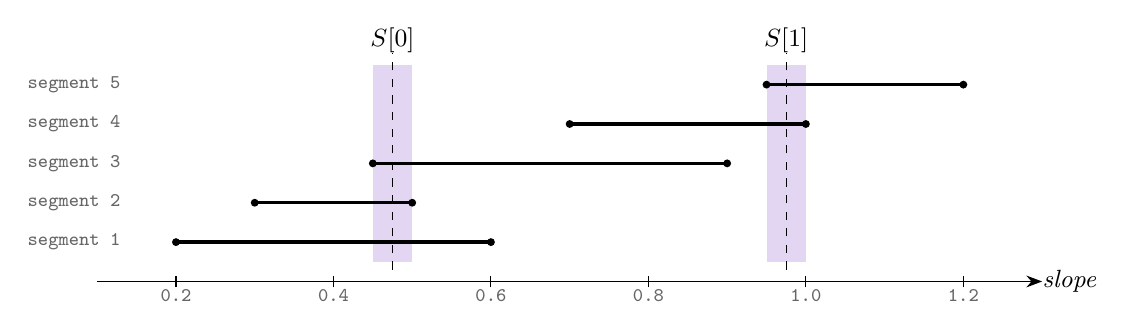
\begin{tikzpicture}[ads,x=100mm,y=5mm]
  \draw[->] (0.1,0) -- (1.3,0) node[right,var] {slope};
  \foreach \x in {0.2,0.4,0.6,0.8,1.0,1.2} {\draw (\x,-0.15) -- (\x,0.15);
    \node[index,below=1mm] at (\x,0) {\x};}
  \fill[adsTouched,opacity=0.7] (0.45,0.5) rectangle (0.5,5.5);
  \fill[adsTouched,opacity=0.7] (0.95,0.5) rectangle (1.0,5.5);
  \foreach \a/\b/\y/\k in {0.2/0.6/1/1,0.3/0.5/2/2,0.45/0.9/3/3,0.7/1.0/4/4,0.95/1.2/5/5}{
    \draw[very thick] (\a,\y) -- (\b,\y);
    \fill (\a,\y) circle (0.5mm); \fill (\b,\y) circle (0.5mm);
    \node[index,anchor=east] at (0.13,\y) {segment \k};}
  \draw[dashed] (0.475,0.3) -- (0.475,5.8) node[above,var] {$S[ 0 ]$};
  \draw[dashed] (0.975,0.3) -- (0.975,5.8) node[above,var] {$S[ 1 ]$};
\end{tikzpicture}
\end{document}
